%% -*- coding: utf-8 -*-
\documentclass[12pt,a4paper]{scrartcl} 
\usepackage[utf8]{inputenc}
\usepackage[english,russian]{babel}
\usepackage{indentfirst}
\usepackage{misccorr}
\usepackage{graphicx}
\usepackage{amsmath}
\usepackage{pgfplots}
\pgfplotsset{compat=1.9}

\begin{document}
\begin{titlepage}
  \begin{center}
    \large




    \vspace{0.5cm}

    Санкт-Петербургский политехнический университет Петра Великого
    \vspace{0.25cm}
    
    Институт компьютерных наук и технологий
    
    Программная инженерия
    \vfill

    \textsc{Лабораторная работа №4}\\[5mm]
    \bigskip
    {\LARGE Тема: Определение опций оптимизации,\\
      для приложения}
  \bigskip
    
    
\end{center}
\vfill

 \newlength{\ML}
\settowidth{\ML}{«\underline{\hspace{0.7cm}}» \underline{\hspace{2cm}}}
\hfill\begin{minipage}{0.5\textwidth}
Работу выполнил студент
  \underline{\hspace{\ML}} А.\,С.~Авферонок\\
1 курс группа № в13534/22\\
  «\underline{\hspace{0.7cm}}» \underline{\hspace{2cm}} 2019 г.
\end{minipage}%
\bigskip
\vfill
 \newlength{\ML}

\settowidth{\ML}{«\underline{\hspace{0.7cm}}» \underline{\hspace{2cm}}}
\hfill\begin{minipage}{0.5\textwidth}
  Преподователь\\
  \underline{\hspace{\ML}} А.\,В.~Петров\\
  «\underline{\hspace{0.7cm}}» \underline{\hspace{2cm}} 2019 г.
\end{minipage}%
\bigskip
\vfill

\begin{center}
  Санкт-Петербург, 2019 г.
\end{center}
\end{titlepage}
\newpage
\begin{center}
    {\LARGE Постановка задачи}
\end{center}
\par
Цель работы - написать сценарий, который будет компелировать программу с разными уровнями оптимизации, 
вычисление времени работы программы и вычисление занимаемого исполняемым файлом дискового пространства.
Сценарий должен принемать имя исходного файла, а время работы исполняемого файла должно быть больше 20 
сейнд.

\newpage
\begin{center}
    {\LARGE Ход выполнения работы}
\end{center}
\par
Для выявления лучшей оптимизации необходимо было написать программу на языке С.
 С условием, что время работы исполняемого файла будет больше 20 секунд.
Было выбранно приложение со следующим исходным кодом:

%Было выбранно приложение с исходным кодом
%время выполнения которого без оптимизации занимало 20+секунд
%Для выявления лучшей оптимизации 
%Исходный код компелируемого приложения:
\begin{verbatim}
    #include <stdio.h>
    double powern (double d, float n) {
        double x = 1.0;
	unsigned j;
	for (j = 1; j <= n; j++)
	    x *= d;
	return x;
    }

    int main (void) {
	double sum = 0.0;
	float i;
	for (i = 1; i <= 1000000; i=i+10)
	{
	    sum += powern (i, i / 5);
	}
	printf ("sume = %g\n", sum);
	return 0;
    }
\end{verbatim}
Время работы его исполняемого файла составли 24,357 секнды, что удовлетовряет условию из постановки задачи.
\par
Далее необходимо было составить сценарий для компеляции выбранного исходного кода и вывода результатов
 времени исполнения и размера исполняемого файла. Текст сценария предоставлен в листнинге.
\par 
Входе компеляций исходного файла были перебранны основные ключи компиляции O0, Os, O1, O2, O3, 
O2 -march=native, O3 -march=native, O2 -march=native -funroll-loops,O3 -march=native -funroll-loops.
Результаты времени исполнения и размера исполняемого файла с использованием разных ключей
 представленны в таблице 1.
\newpage
\begin{center}
\caption{Таблица 1: Результат компиляций с основными ключами}\\
\begin{tabular}{| l | l | l |}
\hline
Ключ оптимизации & Время исполнения, сек & Размер, байт  \\ \hline
O0 & 24,357 & 8672\\
Os & 10,940 & 8672\\
O1 & 10,711 & 8672\\
O2 & 10,693 & 8672\\
O3 & 10,615 & 8672\\
O2 -march=native&	10,588&	8672\\
O3 -march=native &	10,697	&8672\\
O2 -march=native -funroll-loops&	11,026	&8672\\
O3 -march=native -funroll-loops&	10,662	&8672\\
\hline
\end{tabular}\\
\end{center}
\par
Было выявленно, что исполняемы фаил полученный в ходе компиляции с использованием ключа оптимизации
O2 -march=native, исполняется быстрее всех, по этому он был выбран в качестве оптимальной опции.
\par
%Далее прдеставлена таблица и график для наглядного сравнения параметов исполняемого файла, сформированного по резултатом работы сценария.
Далее необходимо было выбрать провести оптимизацию с оптимальной опцией и межпроцедурной оптимезацией и
оптимеацией времени компоновки. Результаты времени исполнения и размера исполняемого файла представленны в
 таблице 2.

\begin{center}
\caption{Таблица 2: Результаты компиляций}
\begin{tabular}{| l | l | l |}
\hline
Ключ оптимизации & Время исполнения, сек & Размер, байт  \\ \hline
O2 -march=native -flto&	10,749	&8608\\
O2 -march=native -fipa-reference&	10,595	&8672\\
\hline
\end{tabular}\\
\end{center}
Было выявленно, что исполняемы фаил полученный в ходе компиляции с использованием ключа оптимизации
O2 -march=native -flto, занимет меньше всех места на дисковом пространсве.
\par

Далее необходимо было выбрать провести оптимизацию с оптимальной опцией и оптимизацией с обратной
связью. Результаты времени исполнения и размера исполняемого файла представленны в таблице 3.

\begin{center}
\caption{Таблица 3: Результаты компиляций}
\begin{tabular}{| l | l | l |}
\hline
Ключ оптимизации & Время исполнения, сек & Размер, байт  \\ \hline
O2 -march=native -fprofile-generate& 10,601	&28688\\
O2 -march=native -fprofile-use&	10,558	&8608\\
\hline
\end{tabular}\\
\end{center}
Было выявленно, что исполняемы фаил полученный в ходе компиляции с использованием ключа оптимизации
O2 -march=native -fprofile-generate, занимет больше всех места на дисковом пространсве и он был исключен
из испытаний, а компиляция с ключем O2 -march=native -fprofile-use дала прирост во времени исполнения.
\par
Получив оптимальные опции оптимизации и обратной связью и межпроцедурной оптимизацией времени, 
было решено объеденить в едино для выяления наилучшего резултата.
 Результаты времени исполнения и размера исполняемого файла представленны в таблице 4.
\begin{center}
\caption{Таблица 4: Результаты компиляций}
\begin{tabular}{| l | l | l |}
\hline
Ключ оптимизации & Время исполнения, сек & Размер, байт  \\ \hline
O2 -march=native -flto -fprofile-use&	10,558	&8608\\
\hline
\end{tabular}\\
\end{center}
Были выявлены наилучшие ключи оптимизации для компиляции выбранного исходного кода.
\par
На рисунке 1 можно наглядно увидить соотношение времени работы исполняемого файла в зависимости от 
ключа оптимизации.
\begin{center}
%\parindent=1cm
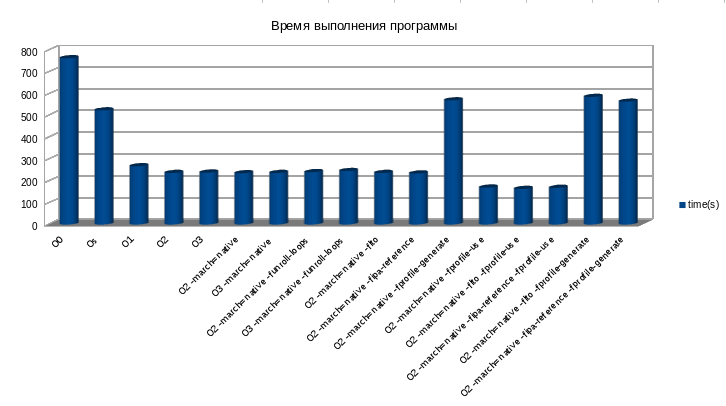
\includegraphics[width=\linewidth]{time.PNG}
\caption{Рисунок 1. Отношение времени к ключу}
\end{center}
На рисунке 2 можно наглядно увидить соотношение занимемого обмема на диске исполняемого файла в зависимости от 
ключа оптимизации.
\begin{center}
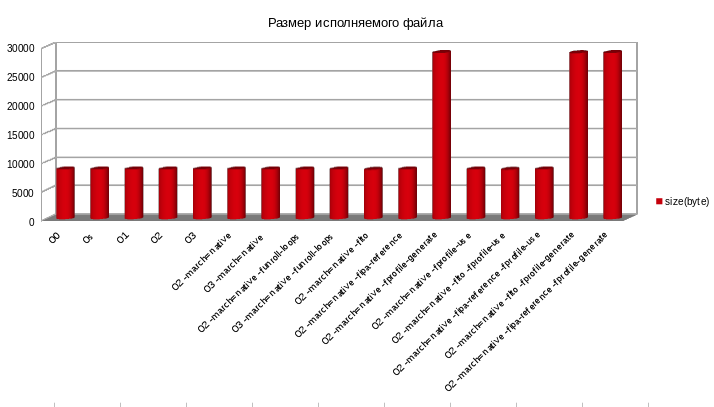
\includegraphics[width=\linewidth]{size.PNG}
\caption{Рисунок 2. Отношение размера к ключу}
\end{center}
\par
\newpage
\begin{center}
    {\LARGE Заключение}
\end{center}
\par
Вывод, в результате выполнения лабораторной работы было выявленно, 
что размер файла не изменялся до использования межпроцедурной
оптимизацией, оптимизацией времени компоновки и оптимизацией с обратной
связью. По этому ключ "O2 -march=native" исполнился за самый короткий промежуток, 10,588 секунд и он был выбран для дальнейшего спользования. \\
\par
Исполняемый фаил занимает меньший объем дискового пространства используя ключ межпроцедурной
оптимизацией "O2 -march=native -flto", 8608 байт, а сильное увеличение размера файла получилось используя ключь оптимизации с
обратной связью "O2 -march=native -fprofile-generate", 28688 байт. \\
\par
Но используя тоже ключ оптимизации с обратной связью "O2 -march=native -fprofile-use" программа исполнилась начительно быстрее, за 10,558 секунд при этом размер занимаемого дискового пространства файлом остался стандартным, 8672 байт.\\
Исходя из этого для достижения максимально оптимизированного решения было выбранно, сгруппировать ключи оптемизации в один.
\par
В итоге, самым быстрм и малозатратным объема диска стал ключ "O2 -march=native -flto -fprofile-use", время исполнения файла 10,558 секунды, размер занимаемого дискового пространства исполняемым файлом 8608 байт.
\\
\newpage
\begin{center}
    {\LARGE Листинг}
\end{center}
Сценарий:
\begin{verbatim}
#!/bin/bash

name=$1

gcc -Wall -O0 $1
echo "-O0"
out="$(time ./a.out)"
by="$(du -b a.out)"
echo "byte :$by"

gcc -Wall -Os $1
echo "-Os"
out="$(time ./a.out)"
by="$(du -b a.out)"
echo "byte :$by"

gcc -Wall -O1 $1
echo "-O1"
out="$(time ./a.out)"
by="$(du -b a.out)"
echo "byte :$by"

gcc -Wall -O2 $1
echo "-O2"
out="$(time ./a.out)"
by="$(du -b a.out)"
echo "byte :$by"

gcc -Wall -O3 $1
echo "-O3"
out="$(time ./a.out)"
by="$(du -b a.out)"
echo "byte :$by"

gcc -Wall -O2 -march=native $1
echo "-O2 -march=native"
out="$(time ./a.out)"
by="$(du -b a.out)"
echo "byte :$by"

gcc -Wall -O3 -march=native $1
echo "-O3 -march=native"
out="$(time ./a.out)"
by="$(du -b a.out)"
echo "byte :$by"

gcc -Wall -O2 -march=native -funroll-loops $1
echo "-O2 -march=native -funroll-loops"
out="$(time ./a.out)"
by="$(du -b a.out)"
echo "byte :$by"

gcc -Wall -O3 -march=native -funroll-loops $1
echo "-O3 -march=native -funroll-loops"
out="$(time ./a.out)"
by="$(du -b a.out)"
echo "byte :$by"

gcc -Wall -O2 -march=native -flto $1
out="$(time ./a.out)"
by="$(du -b a.out)"
echo "-O2 -march=native -flto"
echo "byte :$by"

gcc -Wall -O2 -march=native -fipa-reference $1
out="$(time ./a.out)"
by="$(du -b a.out)"
echo "-O2 -march=native -fipa-reference"
echo "byte :$by"

gcc -Wall -O2 -march=native -fprofile-generate $1
out="$(time ./a.out)"
by="$(du -b a.out)"
echo "-O2 -march=native -fprofile-generate"
echo "byte :$by"

gcc -Wall -O2 -march=native -fprofile-use $1
out="$(time ./a.out)"
by="$(du -b a.out)"
echo "-O2 -march=native -fprofile-use"
echo "byte :$by"

gcc -Wall -O2 -march=native -flto -fprofile-use $1
out="$(time ./a.out)"
by="$(du -b a.out)"
echo "-O2 -march=native -flto -fprofile-use"
echo "byte :$by"

gcc -Wall -O2 -march=native -fipa-reference -fprofile-use $1
out="$(time ./a.out)"
by="$(du -b a.out)"
echo "-O2 -march=native -fipa-reference -fprofile-use"
echo "byte :$by"

gcc -Wall -O2 -march=native -flto -fprofile-generate $1
out="$(time ./a.out)"
by="$(du -b a.out)"
echo "-O2 -march=native -flto -fprofile-generate"
echo "byte :$by"

gcc -Wall -O2 -march=native -fipa-reference -fprofile-generate $1
out="$(time ./a.out)"
by="$(du -b a.out)"
echo "-O2 -march=native -fipa-reference -fprofile-generate"
echo "byte :$by"
\end{verbatim}

\end{document}
